\section{Практическая часть}

\subsection{XSpider}

\begin{figure}[H]
	\centering
	\caption{Результат сканирования XSpider}
	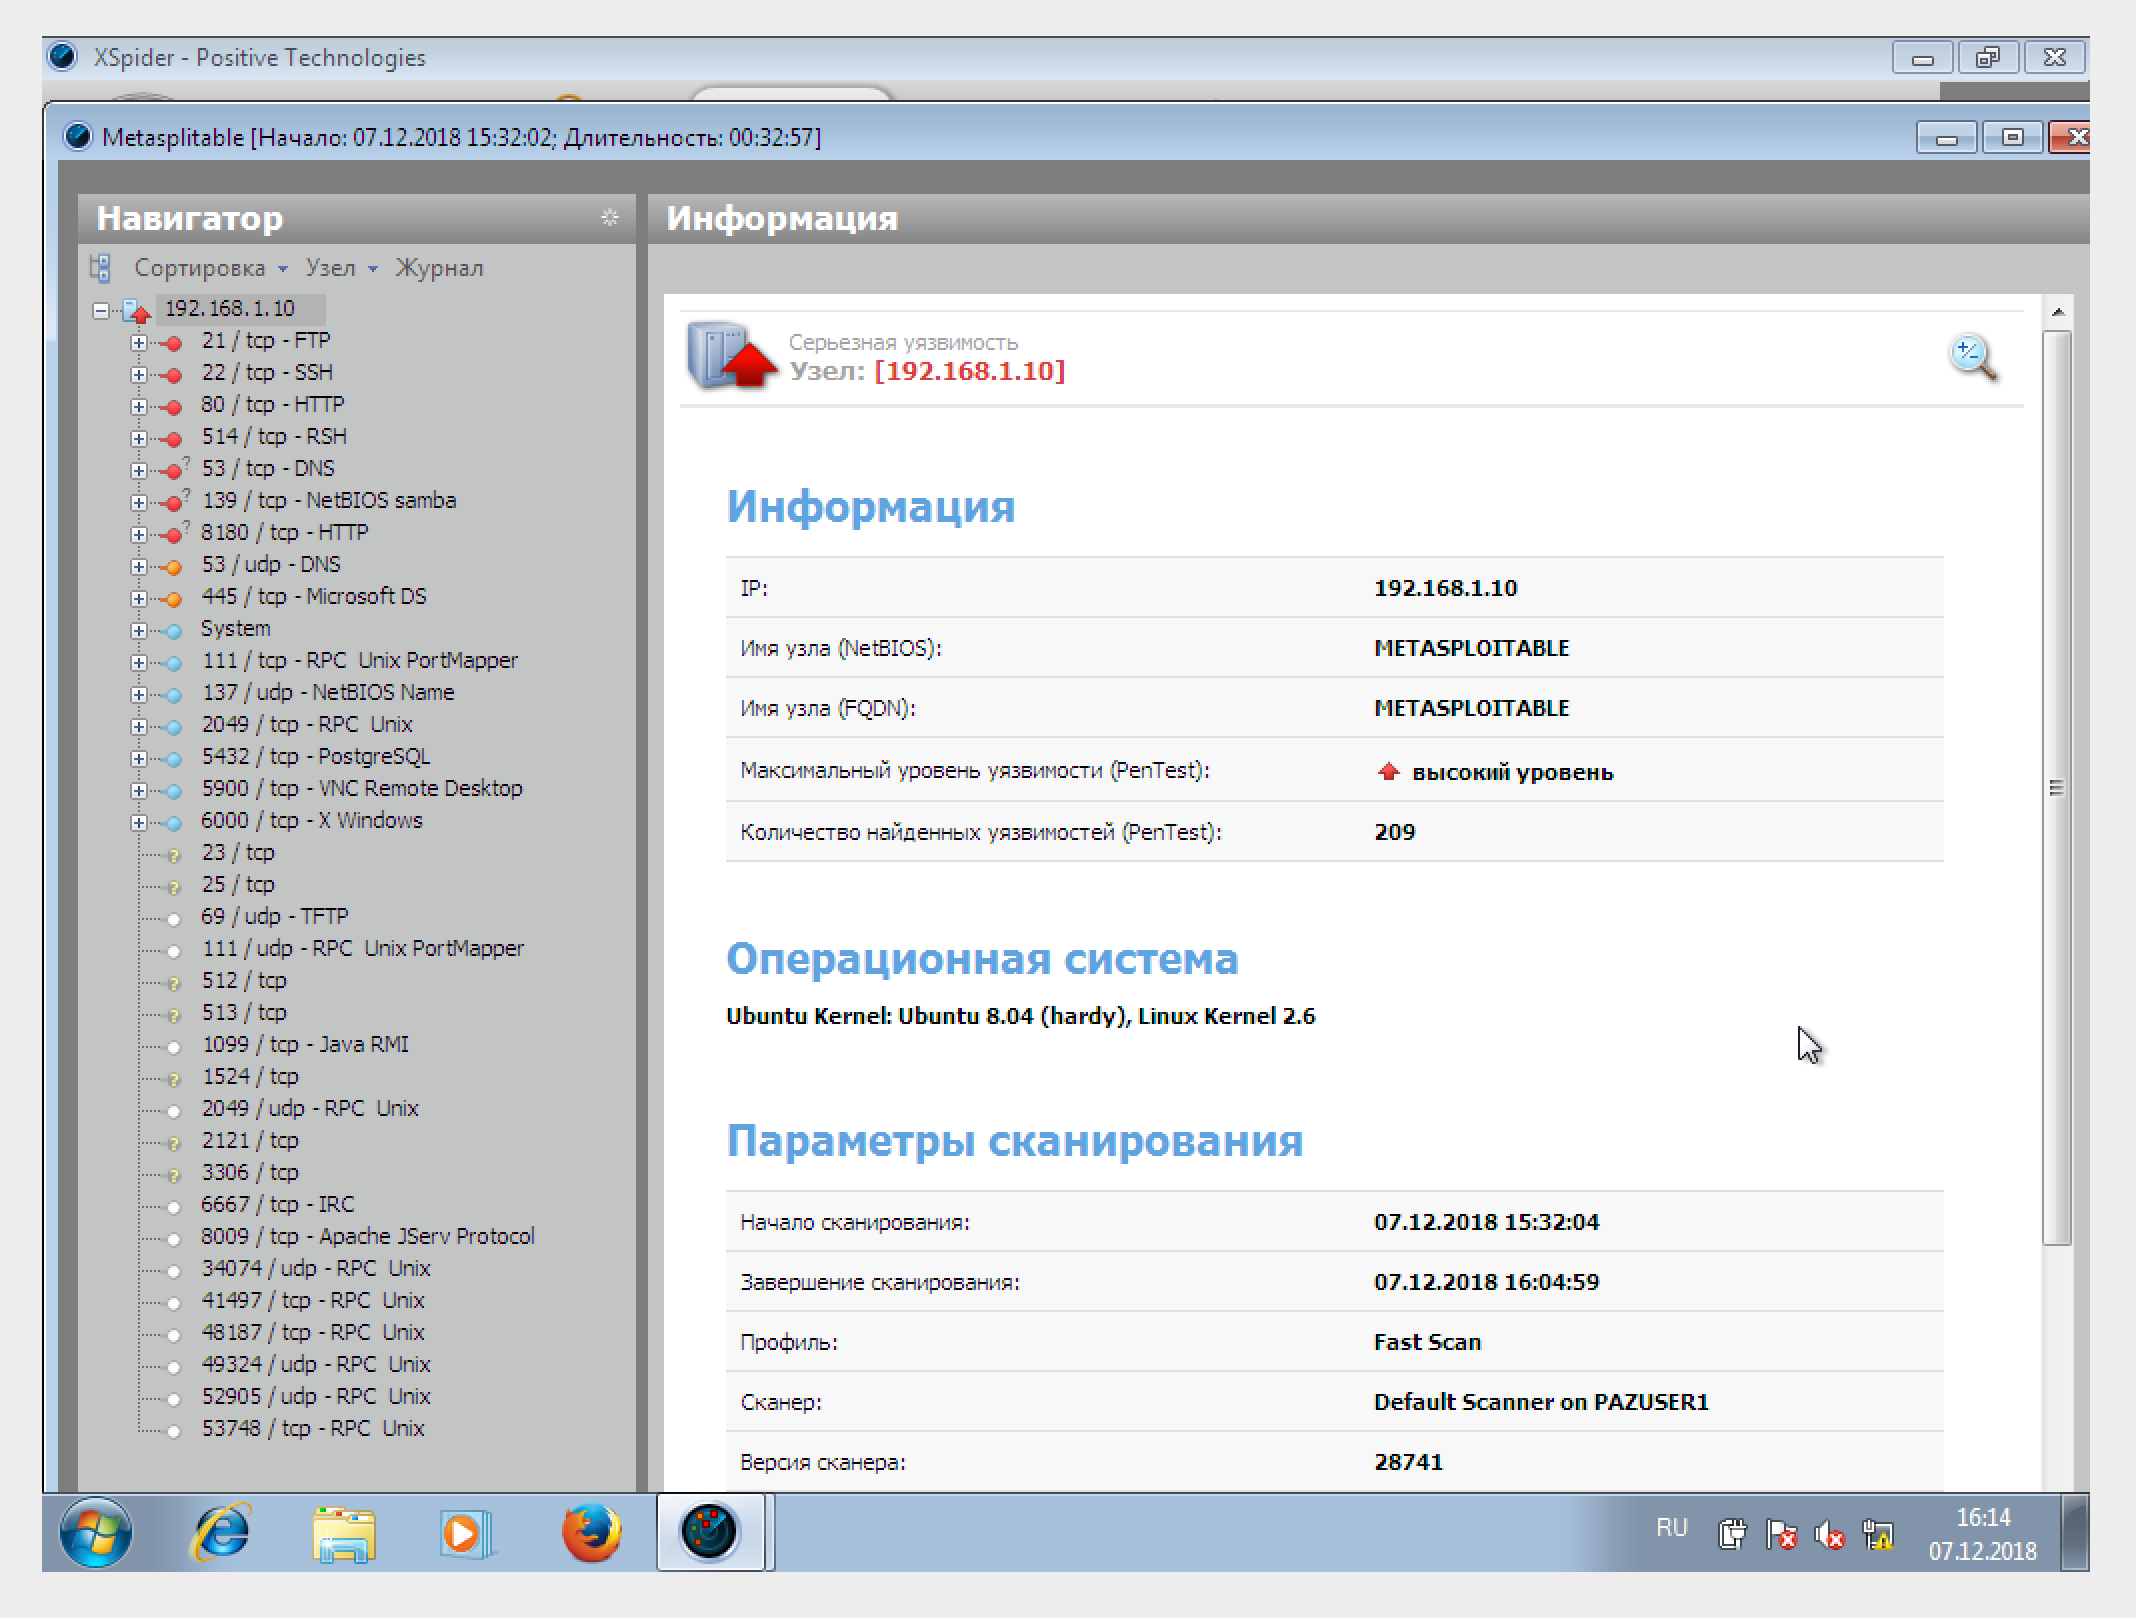
\includegraphics[width=.9\textwidth]{img/spider-result.png}
\end{figure}

\begin{table}[H]
	\centering
	\caption{Результаты сканирования XSpider}
	\begin{tabular}{ccc}
		\hline
		\multicolumn{1}{|c|}{Порт}  & \multicolumn{1}{c|}{Обнаруженный сервис}         & \multicolumn{1}{c|}{Уровень обнаруженной уязвимости} \\ \hline
		\multicolumn{1}{|c|}{21}    & \multicolumn{1}{c|}{vsFTPd 2.3.4}                & \multicolumn{1}{c|}{Высокий}                         \\ \hline
		\multicolumn{1}{|c|}{22}    & \multicolumn{1}{c|}{SSH-2.0-OpenSSH\_4.7p1}      & \multicolumn{1}{c|}{Высокий}                         \\ \hline
		\multicolumn{1}{|c|}{23}    & \multicolumn{1}{c|}{?}                           & \multicolumn{1}{c|}{Не обнаружена}                   \\ \hline
		\multicolumn{1}{|c|}{53}    & \multicolumn{1}{c|}{Bind}                        & \multicolumn{1}{c|}{Высокий}                         \\ \hline
		\multicolumn{1}{|c|}{69}    & \multicolumn{1}{c|}{?}                           & \multicolumn{1}{c|}{Не обнаружена}                   \\ \hline
		\multicolumn{1}{|c|}{80}    & \multicolumn{1}{c|}{Apache+PHP}                  & \multicolumn{1}{c|}{Высокий}                         \\ \hline
		\multicolumn{1}{|c|}{111}   & \multicolumn{1}{c|}{?}                           & \multicolumn{1}{c|}{Не обнаружена}                   \\ \hline
		\multicolumn{1}{|c|}{137}   & \multicolumn{1}{c|}{?}                           & \multicolumn{1}{c|}{Не обнаружена}                   \\ \hline
		\multicolumn{1}{|c|}{139}   & \multicolumn{1}{c|}{Samba}                       & \multicolumn{1}{c|}{Высокий}                         \\ \hline
		\multicolumn{1}{|c|}{445}   & \multicolumn{1}{c|}{Microsoft Directory Service} & \multicolumn{1}{c|}{Средний}                         \\ \hline
		\multicolumn{1}{|c|}{512}   & \multicolumn{1}{c|}{?}                           & \multicolumn{1}{c|}{Не обнаружена}                   \\ \hline
		\multicolumn{1}{|c|}{513}   & \multicolumn{1}{c|}{?}                           & \multicolumn{1}{c|}{Не обнаружена}                   \\ \hline
		\multicolumn{1}{|c|}{514}   & \multicolumn{1}{c|}{rsh}                         & \multicolumn{1}{c|}{Высокий}                         \\ \hline
		\multicolumn{1}{|c|}{1099}  & \multicolumn{1}{c|}{Java RMI}                    & \multicolumn{1}{c|}{Не обнаружена}                   \\ \hline
		\multicolumn{1}{|c|}{1524}  & \multicolumn{1}{c|}{?}                           & \multicolumn{1}{c|}{Не обнаружена}                   \\ \hline
		\multicolumn{1}{|c|}{2049}  & \multicolumn{1}{c|}{NFS}                         & \multicolumn{1}{c|}{Не обнаружена}                   \\ \hline
		\multicolumn{1}{|c|}{2121}  & \multicolumn{1}{c|}{?}                           & \multicolumn{1}{c|}{Не обнаружена}                   \\ \hline
		\multicolumn{1}{|c|}{3306}  & \multicolumn{1}{c|}{?}                           & \multicolumn{1}{c|}{Не обнаружена}                   \\ \hline
		\multicolumn{1}{|c|}{5432}  & \multicolumn{1}{c|}{PostgreSQL}                  & \multicolumn{1}{c|}{Не обнаружена}                   \\ \hline
		\multicolumn{1}{|c|}{5900}  & \multicolumn{1}{c|}{VNC Remote Desktop}          & \multicolumn{1}{c|}{Не обнаружена}                   \\ \hline
		\multicolumn{1}{|c|}{6000}  & \multicolumn{1}{c|}{X Windows}                   & \multicolumn{1}{c|}{Не обнаружена}                   \\ \hline
		\multicolumn{1}{|c|}{6667}  & \multicolumn{1}{c|}{IRC}                         & \multicolumn{1}{c|}{Не обнаружена}                   \\ \hline
		\multicolumn{1}{|c|}{8009}  & \multicolumn{1}{c|}{Apache JServ Protocol}       & \multicolumn{1}{c|}{Не обнаружена}                   \\ \hline
		\multicolumn{1}{|c|}{8180}  & \multicolumn{1}{c|}{Apache Tomcat}               & \multicolumn{1}{c|}{Не обнаружена}                   \\ \hline
		\multicolumn{1}{|c|}{34074} & \multicolumn{1}{c|}{?}                           & \multicolumn{1}{c|}{Не обнаружена}                   \\ \hline
		\multicolumn{1}{|c|}{41497} & \multicolumn{1}{c|}{?}                           & \multicolumn{1}{c|}{Не обнаружена}                   \\ \hline
		\multicolumn{1}{|c|}{48187} & \multicolumn{1}{c|}{?}                           & \multicolumn{1}{c|}{Не обнаружена}                   \\ \hline
		\multicolumn{1}{|c|}{49324} & \multicolumn{1}{c|}{?}                           & \multicolumn{1}{c|}{Не обнаружена}                   \\ \hline
		\multicolumn{1}{|c|}{52905} & \multicolumn{1}{c|}{?}                           & \multicolumn{1}{c|}{Не обнаружена}                   \\ \hline
		\multicolumn{1}{l}{}        & \multicolumn{1}{l}{}                             & \multicolumn{1}{l}{}                                
	\end{tabular}
\end{table}



Из 30-ти открытых портов:

\begin{itemize}
	\item Определено 15 сервисов
	\item Найдено 7 значимых уязвимостей
\end{itemize}


\subsection{Nessus}

\begin{figure}[H]
	\centering
	\caption{Результат сканирования Nessus}
	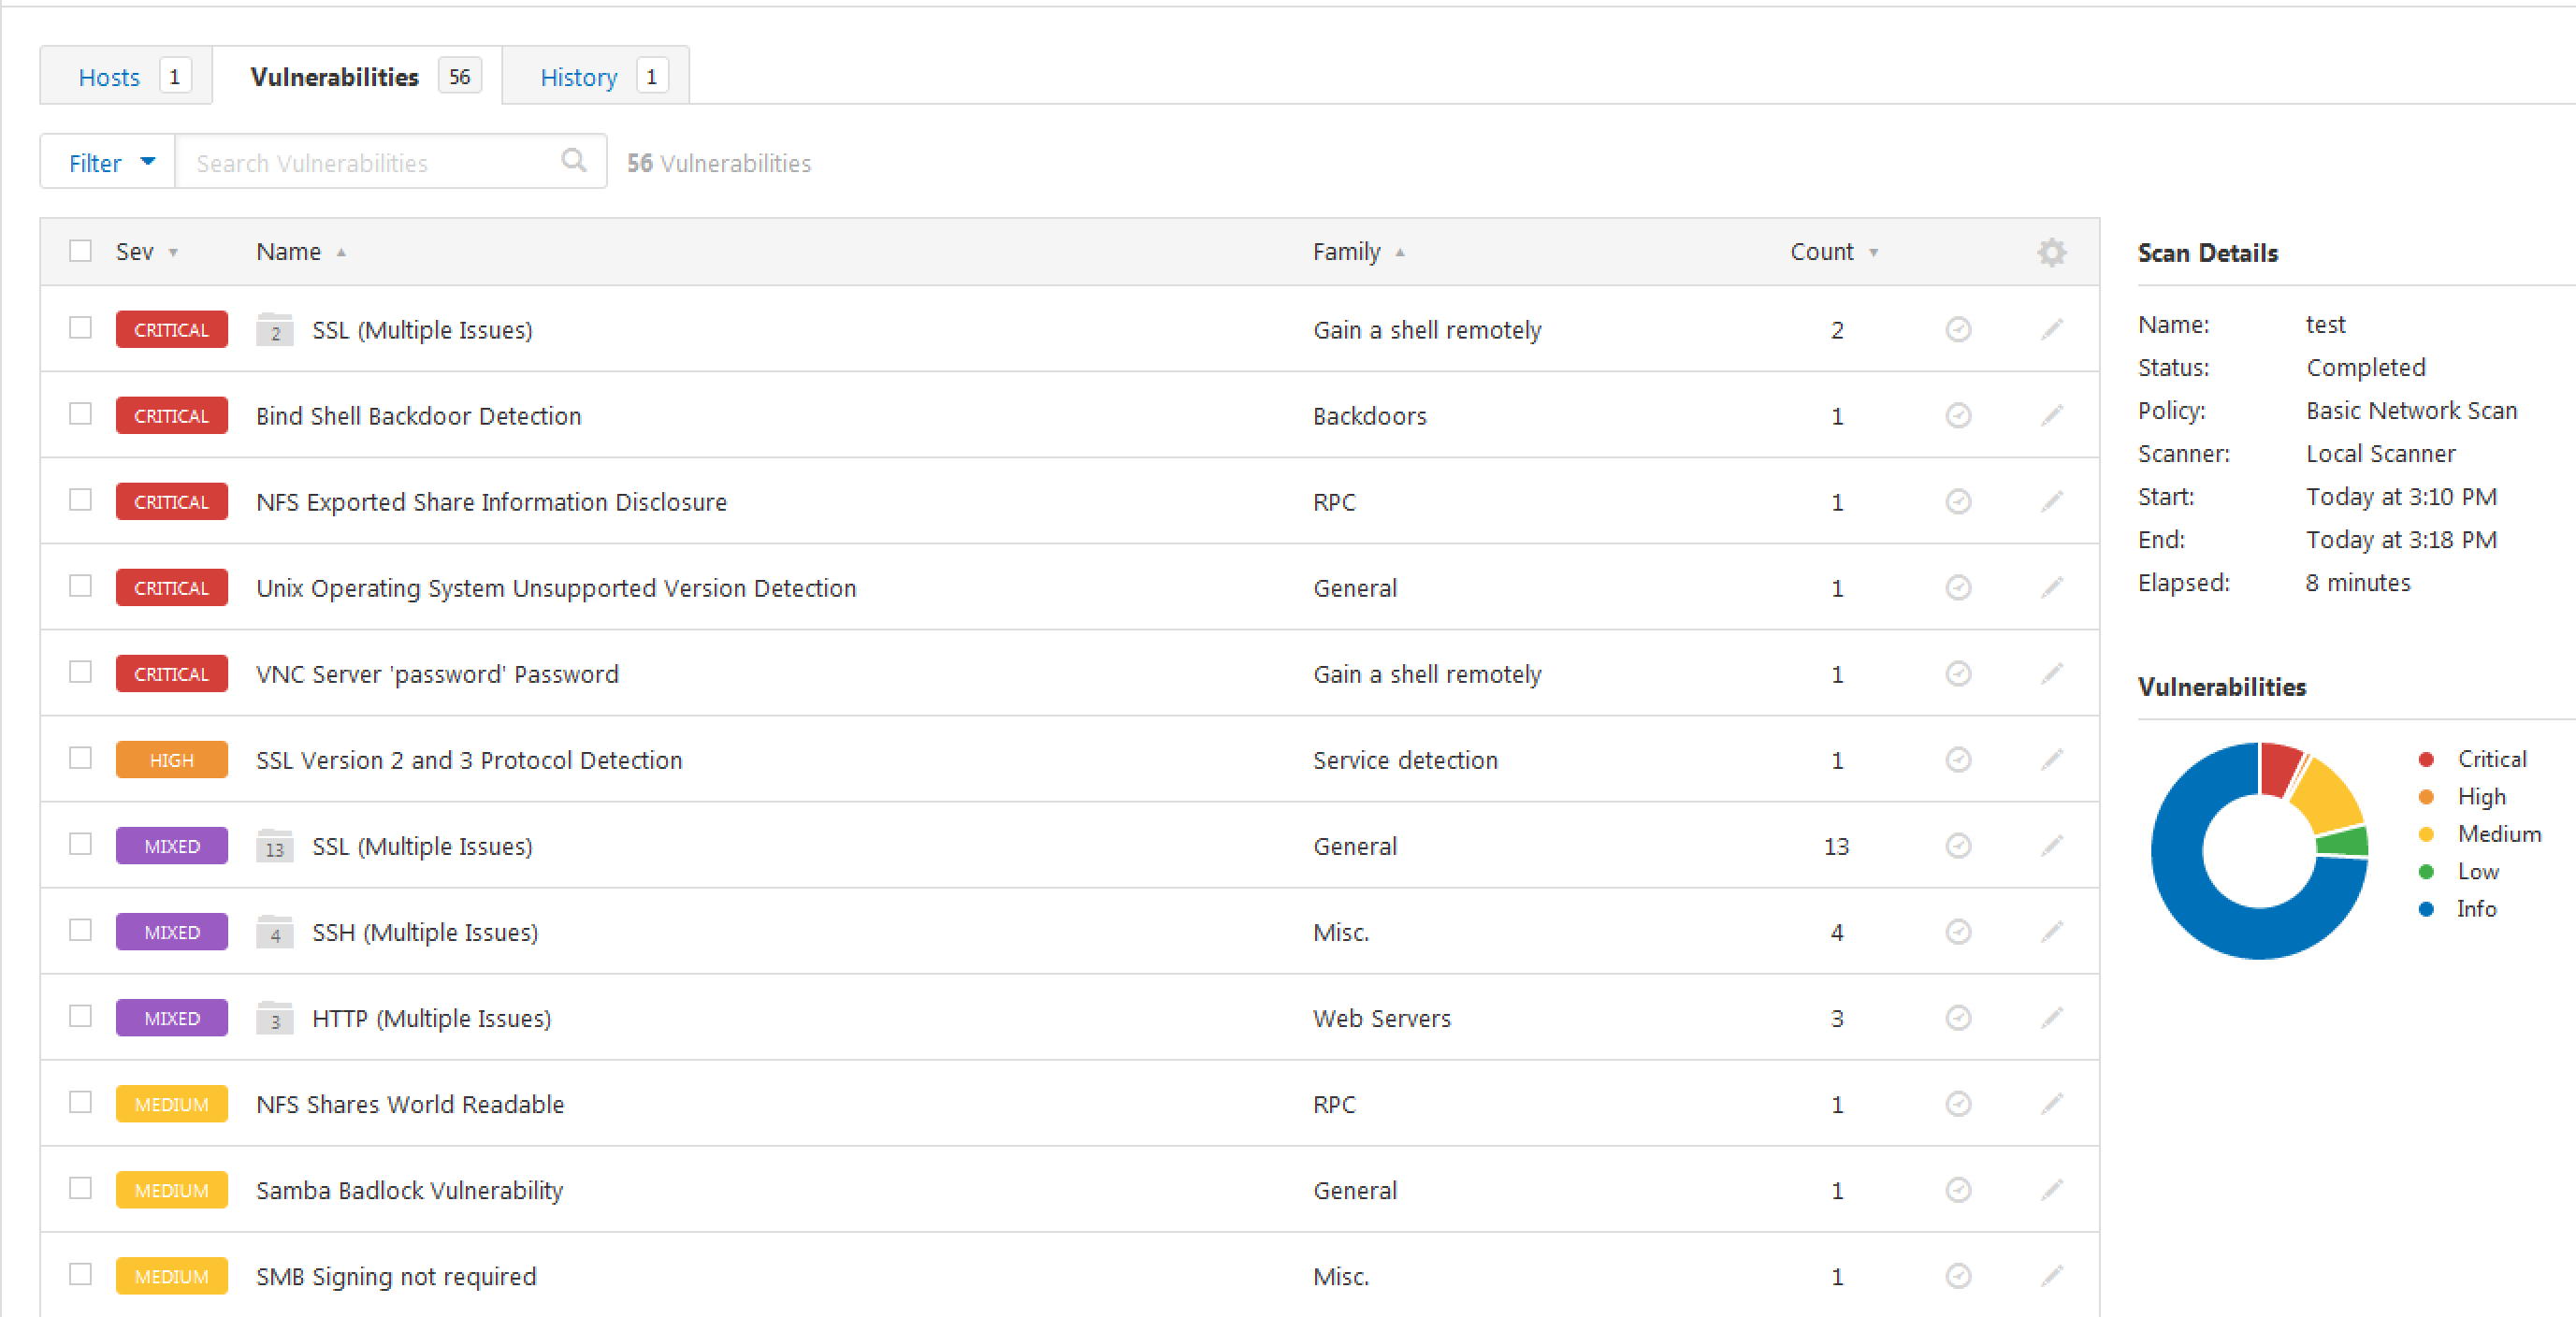
\includegraphics[width=.9\textwidth]{img/nessus-result.png}
\end{figure}

Из 30-ти открытых портов:

\begin{itemize}
	\item Определено 30 сервисов
	\item Найдено 7 значимых уязвимостей
\end{itemize}

\subsection{nmap}

Вне категорий. Находит всё.

\lstinputlisting{src/nmap.in}


\subsection{Сводная таблица}

\begin{table}[H]
	\centering
	\resizebox{\textwidth}{!}{%
		\begin{tabular}{cccl}
			\hline
			\multicolumn{1}{|c|}{}      & \multicolumn{1}{c|}{Сервис}                                      & \multicolumn{1}{c|}{Обнаружено XSpider} & \multicolumn{1}{l|}{Обнаружено Nessus} \\ \hline
			\multicolumn{1}{|c|}{21}    & \multicolumn{1}{c|}{vsFTPd 2.3.4}                                & \multicolumn{1}{c|}{Да}                 & \multicolumn{1}{l|}{}                  \\ \hline
			\multicolumn{1}{|c|}{22}    & \multicolumn{1}{c|}{SSH-2.0-OpenSSH\_4.7p1}                      & \multicolumn{1}{c|}{Да}                 & \multicolumn{1}{l|}{}                  \\ \hline
			\multicolumn{1}{|c|}{23}    & \multicolumn{1}{c|}{Linux telnetd}                               & \multicolumn{1}{c|}{}                   & \multicolumn{1}{l|}{}                  \\ \hline
			\multicolumn{1}{|c|}{53}    & \multicolumn{1}{c|}{ISC BIND 9.4.2}                              & \multicolumn{1}{c|}{Да}                 & \multicolumn{1}{l|}{Да}                \\ \hline
			\multicolumn{1}{|c|}{69}    & \multicolumn{1}{c|}{?}                                           & \multicolumn{1}{c|}{}                   & \multicolumn{1}{l|}{}                  \\ \hline
			\multicolumn{1}{|c|}{80}    & \multicolumn{1}{c|}{Apache+PHP}                                  & \multicolumn{1}{c|}{Да}                 & \multicolumn{1}{l|}{}                  \\ \hline
			\multicolumn{1}{|c|}{111}   & \multicolumn{1}{c|}{rpcbind}                                     & \multicolumn{1}{c|}{}                   & \multicolumn{1}{l|}{}                  \\ \hline
			\multicolumn{1}{|c|}{137}   & \multicolumn{1}{c|}{?}                                           & \multicolumn{1}{c|}{}                   & \multicolumn{1}{l|}{}                  \\ \hline
			\multicolumn{1}{|c|}{139}   & \multicolumn{1}{c|}{Sambasmbd 3.X - 4.X (workgroup: WORKGROUP)}  & \multicolumn{1}{c|}{Да}                 & \multicolumn{1}{l|}{}                  \\ \hline
			\multicolumn{1}{|c|}{445}   & \multicolumn{1}{c|}{Samba smbd 3.X - 4.X (workgroup: WORKGROUP)} & \multicolumn{1}{c|}{Да}                 & \multicolumn{1}{l|}{}                  \\ \hline
			\multicolumn{1}{|c|}{512}   & \multicolumn{1}{c|}{netkit-rsh rexecd}                           & \multicolumn{1}{c|}{}                   & \multicolumn{1}{l|}{}                  \\ \hline
			\multicolumn{1}{|c|}{513}   & \multicolumn{1}{c|}{login}                                       & \multicolumn{1}{c|}{}                   & \multicolumn{1}{l|}{}                  \\ \hline
			\multicolumn{1}{|c|}{514}   & \multicolumn{1}{c|}{rsh}                                         & \multicolumn{1}{c|}{Да}                 & \multicolumn{1}{l|}{}                  \\ \hline
			\multicolumn{1}{|c|}{1099}  & \multicolumn{1}{c|}{GNU Classpath grmiregistry}                  & \multicolumn{1}{c|}{}                   & \multicolumn{1}{l|}{}                  \\ \hline
			\multicolumn{1}{|c|}{1524}  & \multicolumn{1}{c|}{Metasploitable root shell}                   & \multicolumn{1}{c|}{}                   & \multicolumn{1}{l|}{}                  \\ \hline
			\multicolumn{1}{|c|}{2049}  & \multicolumn{1}{c|}{NFS}                                         & \multicolumn{1}{c|}{}                   & \multicolumn{1}{l|}{Да}                \\ \hline
			\multicolumn{1}{|c|}{2121}  & \multicolumn{1}{c|}{ProFTPD 1.3.1}                               & \multicolumn{1}{c|}{}                   & \multicolumn{1}{l|}{}                  \\ \hline
			\multicolumn{1}{|c|}{3306}  & \multicolumn{1}{c|}{MySQL 5.0.51a-3ubuntu5}                      & \multicolumn{1}{c|}{}                   & \multicolumn{1}{l|}{}                  \\ \hline
			\multicolumn{1}{|c|}{5432}  & \multicolumn{1}{c|}{PostgreSQLDB 8.3.0 - 8.3.7}                  & \multicolumn{1}{c|}{}                   & \multicolumn{1}{l|}{}                  \\ \hline
			\multicolumn{1}{|c|}{5900}  & \multicolumn{1}{c|}{VNC (protocol 3.3)}                          & \multicolumn{1}{c|}{}                   & \multicolumn{1}{l|}{Да}                \\ \hline
			\multicolumn{1}{|c|}{6000}  & \multicolumn{1}{c|}{X Windows}                                   & \multicolumn{1}{c|}{}                   & \multicolumn{1}{l|}{}                  \\ \hline
			\multicolumn{1}{|c|}{6667}  & \multicolumn{1}{c|}{IRC}                                         & \multicolumn{1}{c|}{}                   & \multicolumn{1}{l|}{}                  \\ \hline
			\multicolumn{1}{|c|}{8009}  & \multicolumn{1}{c|}{Apache JServ Protocol}                       & \multicolumn{1}{c|}{}                   & \multicolumn{1}{l|}{}                  \\ \hline
			\multicolumn{1}{|c|}{8180}  & \multicolumn{1}{c|}{Apache Tomcat}                               & \multicolumn{1}{c|}{}                   & \multicolumn{1}{l|}{}                  \\ \hline
			\multicolumn{1}{|c|}{34074} & \multicolumn{1}{c|}{?}                                           & \multicolumn{1}{c|}{}                   & \multicolumn{1}{l|}{}                  \\ \hline
			\multicolumn{1}{|c|}{41497} & \multicolumn{1}{c|}{?}                                           & \multicolumn{1}{c|}{}                   & \multicolumn{1}{l|}{}                  \\ \hline
			\multicolumn{1}{|c|}{48187} & \multicolumn{1}{c|}{?}                                           & \multicolumn{1}{c|}{}                   & \multicolumn{1}{l|}{}                  \\ \hline
			\multicolumn{1}{|c|}{49324} & \multicolumn{1}{c|}{?}                                           & \multicolumn{1}{c|}{}                   & \multicolumn{1}{l|}{}                  \\ \hline
			\multicolumn{1}{|c|}{52905} & \multicolumn{1}{c|}{?}                                           & \multicolumn{1}{c|}{}                   & \multicolumn{1}{l|}{}                  \\ \hline
			\multicolumn{1}{l}{}        & \multicolumn{1}{l}{}                                             & \multicolumn{1}{l}{}                    &                                       
		\end{tabular}%
	}
\end{table}

Выглядит не особенно убедительно, учитывая, сколько уязвимостей осталось нераспознанными. 

Сухая математика:

\[
\sum_{xspider}=3 \cdot 7 + 2 \cdot 2 + 7 * 1 = 32
\]

\[
\sum_{nessus}=3 \cdot 5 + 1 \cdot 2 + 4 * 1 = 21
\]

Побеждает XSpider.


